%%%%%%%%%%%%%%%%%%%%%%%%%%%%%%%%%%%%%%%%%
% Journal Article
% LaTeX Template
% Version 1.3 (9/9/13)
%
% This template has been downloaded from:
% http://www.LaTeXTemplates.com
%
% Original author:
% Frits Wenneker (http://www.howtotex.com)
%
% License:
% CC BY-NC-SA 3.0 (http://creativecommons.org/licenses/by-nc-sa/3.0/)
%
%%%%%%%%%%%%%%%%%%%%%%%%%%%%%%%%%%%%%%%%%

%----------------------------------------------------------------------------------------
%	PACKAGES AND OTHER DOCUMENT CONFIGURATIONS
%----------------------------------------------------------------------------------------

\documentclass[twoside]{article}

\usepackage{lipsum} % Package to generate dummy text throughout this template


\usepackage[sc]{mathpazo} % Use the Palatino font
\usepackage[T1]{fontenc} % Use 8-bit encoding that has 256 glyphs
\usepackage[utf8]{inputenc}
\linespread{1.05} % Line spacing - Palatino needs more space between lines
\usepackage{microtype} % Slightly tweak font spacing for aesthetics
\usepackage{amsmath}
\usepackage{listings}

\lstset{
    basicstyle=\ttfamily\footnotesize,
    breaklines=true
}


%\usepackage[hmarginratio=1:1,top=32mm,columnsep=20pt]{geometry} % Document margins
\usepackage[margin={1cm,2cm}]{geometry}
\setlength{\columnsep}{1cm}
\usepackage{multicol} % Used for the two-column layout of the document
\usepackage[hang, small,labelfont=bf,up,textfont=it,up]{caption} % Custom captions under/above floats in tables or figures
\usepackage{booktabs} % Horizontal rules in tables
\usepackage{float} % Required for tables and figures in the multi-column environment - they need to be placed in specific locations with the [H] (e.g. \begin{table}[H])
\usepackage{hyperref} % For hyperlinks in the PDF
\usepackage{multirow}

\usepackage{lettrine} % The lettrine is the first enlarged letter at the beginning of the text
\usepackage{paralist} % Used for the compactitem environment which makes bullet points with less space between them

\usepackage{abstract} % Allows abstract customization
\renewcommand{\abstractnamefont}{\normalfont\bfseries} % Set the "Abstract" text to bold
\renewcommand{\abstracttextfont}{\normalfont\small\itshape} % Set the abstract itself to small italic text


\usepackage{graphicx}

\usepackage{tikz}


\newcommand{\rparen}{)}

\usepackage{titlesec} % Allows customization of titles
\renewcommand\thesection{\Roman{section}} % Roman numerals for the sections
%\renewcommand{\thesubsection}{\thesection\hspace{1mm}\alph{subsection}}
\titleformat{\section}[block]{\large\scshape\centering}{\thesection}{1em}{} % Change the look of the section titles
\titleformat{\subsection}[block]{\large}{\thesubsection}{1em}{} % Change the look of the section titles

\usepackage{fancyhdr} % Headers and footers
\pagestyle{fancy} % All pages have headers and footers
\fancyhead{} % Blank out the default header
\fancyfoot{} % Blank out the default footer
\fancyhead[C]{IT3708 Sub-symbolic AI Methods $\bullet$ Project 4 $\bullet$ \date{\today}} % Custom header text
\fancyfoot[RO,LE]{\thepage} % Custom footer text

%----------------------------------------------------------------------------------------
%	TITLE SECTION
%----------------------------------------------------------------------------------------

\title{\vspace{-15mm}\fontsize{18pt}{10pt}\selectfont\textbf{Evolving Continuous Time Recurrent Neural Networks\\for a Beer Tracker Agent - Project Report}} % Article title

\author{
    \large
    \textsc{Mathias Ose \& Øyvind Robertsen} \\ % Your name
    \normalsize Norwegian University of Science \& Technology \\ % Your institution
    \normalsize \href{mailto:mathiabo@stud.ntnu.no}{mathiabo@stud.ntnu.no}, \href{mailto:oyvinrob@stud.ntnu.no}{oyvinrob@stud.ntnu.no} % Your email address
    \vspace{-5mm}
}
\date{}

%----------------------------------------------------------------------------------------

\begin{document}

\maketitle % Insert title

\thispagestyle{fancy} % All pages have headers and footers

%----------------------------------------------------------------------------------------
%	ABSTRACT
%----------------------------------------------------------------------------------------

\begin{abstract}

    \noindent This report describes a solution to Project 4 in the subject IT3708 at NTNU. 
    The purpose of this project is to use an evolutionary algorithm to tune the weights of a continuous time recurrent neural network, which then acts as an agent in a simple game in a 2D world and receives a performance score.
\end{abstract}

%----------------------------------------------------------------------------------------
%	ARTICLE CONTENTS
%----------------------------------------------------------------------------------------

\begin{multicols}{2} % Two-column layout throughout the main article text

    \section{Implementation}
    A phenotype is the representation of the weights of a CTRNN.
    A CTRNN requires more weights than the simple ANN from project 3.
    In addition to matrices that represent arcs crossing between layers,
    there are also internal arcs between the neurons of a layer,
    and each neuron requires two additional paramenters, the \textit{gain} and \textit{time constant}.

    The genotype is a bitstring of size $8 * \text{number of weights}$.
    The conversion to phenotype takes each 8 bit sequence and interprets it as a floating point value between $0.0$ and $1.0$.
    These values are then fitted into matrices that represent the arc weights,
    or assigned as \texttt{g} or \texttt{t} values of neurons,
    and scaled and adjusted to the appropriate range for that weight type.

    The CTRNN implementation is a modified version of the ANN implementation from project 3.
    Neurons are no longer only simple numerical values where input is equal to output,
    but are objects that maintain state and computes output based on input and state.

    At each tick of the simulation the input nodes get either $1$ or $0$ from the sensors.
    They then output some value computed with the input, the previous state, the \textit{gain} and \textit{time constant} parameters and the sigmoid function.
    These values are propagated along the weighted arcs to the next layer,
    where the sum of the inputs to each neuron goes through the same calculation.
    In the CTRNN there are also internal arcs in each non-input layer,
    including arcs from the neuron to itself.
    These are also part of the sum of inputs.

    Once the sensory inputs have propagated their way through the network and the final layer has new output values,
    the agent object uses these values to make a decision about how to act in the Beer Tracker World.
    If the left neuron has a higher value than the right neuron the agent will move left, and vice versa.
    The magnitude of the output decides the magnitude of the movement,
    so an output near $1.0$ means the agent takes 4 steps and an output near $0.0$ means it takes no steps at all.

    \section{Performance}
    \begin{lstlisting}[caption=Awarding points which are used for fitness measure, label=points]
    def capture(self, obj):
        if obj.width >= 5:
            self.points -= 2
        else:
            self.points += 1

    def avoidance(self, obj):
        if obj.width >= 5:
            self.points += 2
        else:
            self.points -= 1

    def fail(self, obj):
        self.points -= 2
    \end{lstlisting}

    \begin{figure}[H]
        \centering
        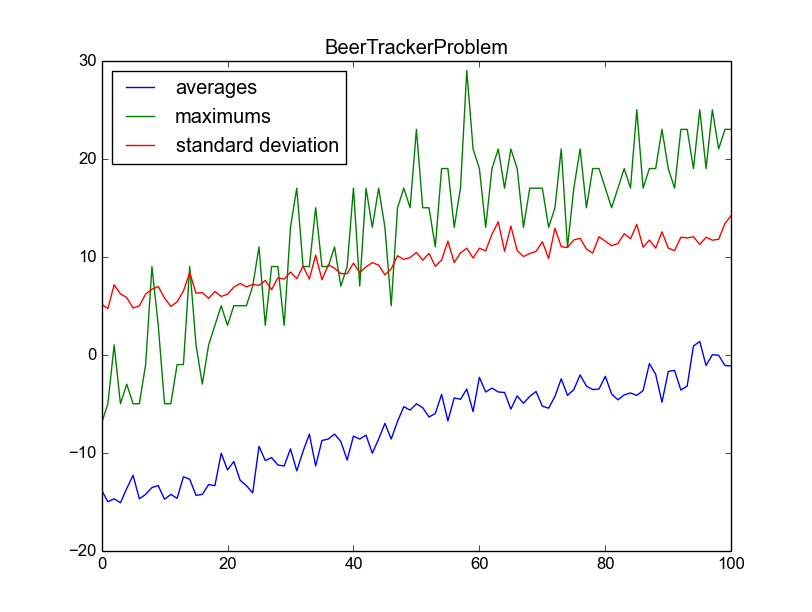
\includegraphics[width=\linewidth]{images/i_like_dis_grap}
        \caption{Standard scenario, 100 generations of evolution}
        \label{standard}
    \end{figure}

    Listing \ref{points} shows how points are awarded.
    It is possible to capture an object, to avoid it, or to fail at either.
    These points are used as the fitness measure, which can be seen evolving in figure \ref{standard}.

    It is more difficult to consistently reproduce the same behavior in this project than it has been in previous projects.
    This is because both the problem and the CTRNN itself are more complex,
    with more variable parameters and more randomness.

    In the standard scenario the most commonly seen evolved behavior is an agent which moves in only one direction.
    It stops and stands still to capture most objects,
    but is usually not very good at avoiding the dangerous objects,
    and often tries to capture big objects as well.

    We have however also seen smarter agents appear sometimes,
    that are able to avoid most dangerous objects,
    while also being able to capture most safe objects.
    These will typically slow down when they find an object,
    and do small steps to "figure out" the size of the object,
    then either stand still if it is safe or accelerate away if not.
    With 1-3 wide objects they stop and wait, with 4-wide objects they move about more because of the lack of long term memory.

    The agent in the "pull" scenario typically acts a lot like the standard agent,
    but uses the pull move instead of standing still and waiting for small objects to drop.
    Sometimes the time recurrency of the network makes it use the pull power two times in rapid succession, because of the recurrency in the network.

    In the no-wrap scenario the most commonly seen behavior is for the agent to move to one of the corners and then just sitting there for the entirety of the simulation.
    We managed to evolve an agent into moving back and forth by increasing the range of the time constant drastically, seen in figure \ref{nowrap}.
    However this agent did not do very well at capturing and avoiding.

    \begin{figure}[H]
        \centering
        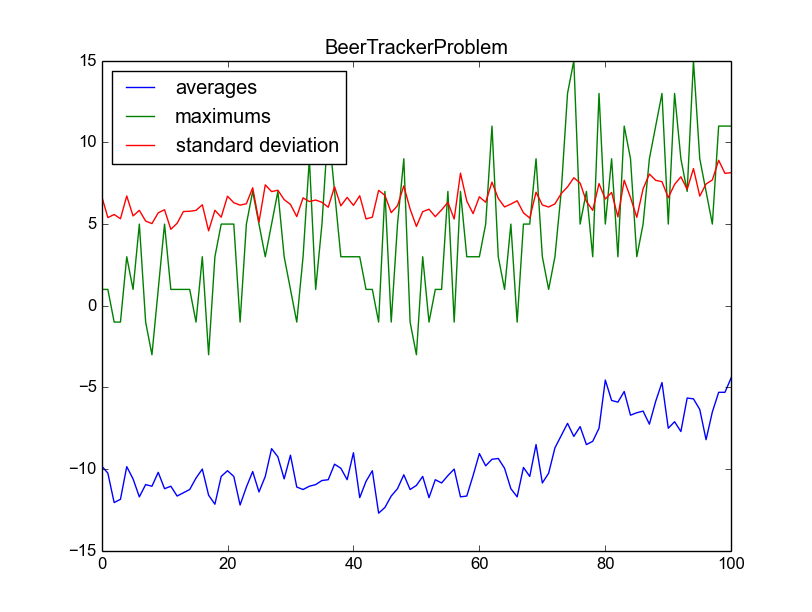
\includegraphics[width=\linewidth]{images/nowrap_highT}
        \caption{Nowrap scenario, 100 generations of evolution}
        \label{nowrap}
    \end{figure}

    \section{Analysis}
    \begin{lstlisting}[caption=Evolved phenotype, label=phenotype]
    {'inter': [array([[-4.60784314, -4.33333333],
            [ 4.41176471,  4.29411765]]), array([[ 2.25490196,  1.54901961],
        [-2.1372549 , -2.96078431]])], 'cross': [array([[ 4.01960784, -0.7254902 ],
                [-3.74509804, -4.33333333],
                [-0.52941176, -1.78431373],
                [ 1.43137255, -1.43137255],
                [ 2.33333333, -4.68627451],
            [-1.03921569, -3.98039216]]), array([[-0.21568627,  3.94117647],
                [-2.49019608, -1.31372549],
    [-4.96078431, -2.76470588]])], 'ts': [1.2980392156862746, 1.192156862745098, 1.192156862745098, 1.192156862745098, 1.1607843137254903, 1.1294117647058823, 1.9607843137254903, 1.396078431372549, 1.1686274509803922], 'gains': [3.9019607843137254, 1.0784313725490196, 3.83921568627451, 3.1333333333333333, 2.6, 3.164705882352941, 1.188235294117647, 2.4117647058823533, 2.7254901960784315]}
    \end{lstlisting}

    The evolved phenotype shown in listing \ref{phenotype} is very good at capturing and avoiding correctly when it finds objects,
    but moves very slowly, so still misses a lot.

\end{multicols}

%\bibliography{references}
%\bibliographystyle{plain}

\end{document}
